\section{Preliminary Results}


After we hold $c$ and $y_C$ constant, we end up with a single PDE. Dropping the spatial term, and analyzing the single ODE we find that the ODE is can be monostable low, in which case the only solution is $0$, monostable high, in which case there is a single steady state solution $\ne 0$ or it can be bistable. See Fig.~\ref{fig::phaseline} for a plot of the single ODE in the various regimes. 
\begin{figure}[h]
\centering
\captionsetup{width=0.9\linewidth}
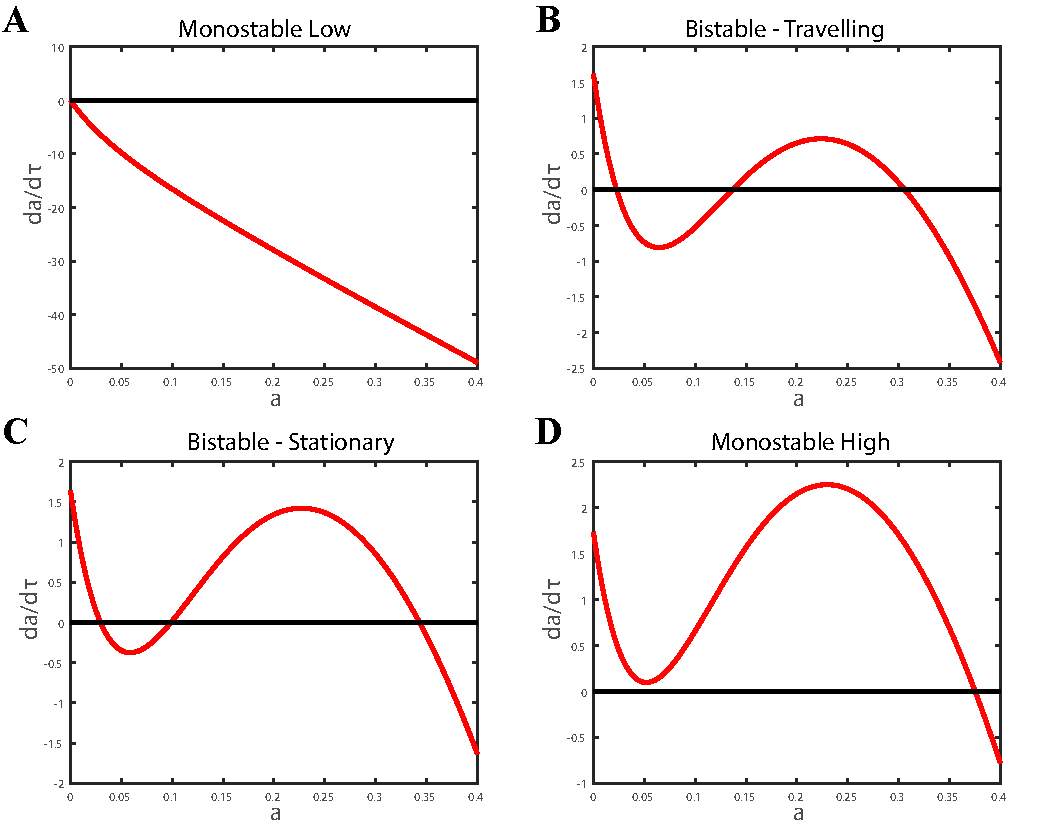
\includegraphics[width=4.5in]{Project2/figs/phaseline.pdf}
\caption{Plot of da/d$t$ vs a for four different parameter sets. A) The monostable zero case, $\Omega = 57$ and $F = 0.95$. B) The bistable ODE-travelling PDE regime, $\Omega = 55$ and $F = 1.2$. C) The  bistable ODE-stationary PDE regime, $\Omega =50 $ and $F = 1.4$. D) The monostable high case,  $\Omega = 45$ and $F = 1.55$.}
\label{fig::phaseline}
\end{figure}

\hspace{6pt}

The non-local Maxwell condition is equal to $0$ in both of the monostable regimes (because $y^- = y^+$), but can be negative or positive in the bistable regime. Returning to the PDE, we don't expect travelling solutions to arise from a monostable regime, but we wish to see for which region of the bistable regime the non-local Maxwell condition predicts travelling solutions. By varying two parameters continuously we can determine these regions. This is shown in Fig.~\ref{fig::NLMC}(A). Here the parameters varied are $\Omega$ which is not present in the single PDE but changes are reflected in $c^{ss}$, and $F$. We plan to create identical plots using other pairs of parameters. The regions shown in Fig.~\ref{fig::NLMC} (A) match up well with the numerical solutions of the PDE as depicted in Eq.~\ref{fig::NLMC} (B), which shows the velocity of the travelling wave solution ($=0$ for a stationary solution).


\begin{figure}[h]
\centering
\captionsetup{width=.9\linewidth}
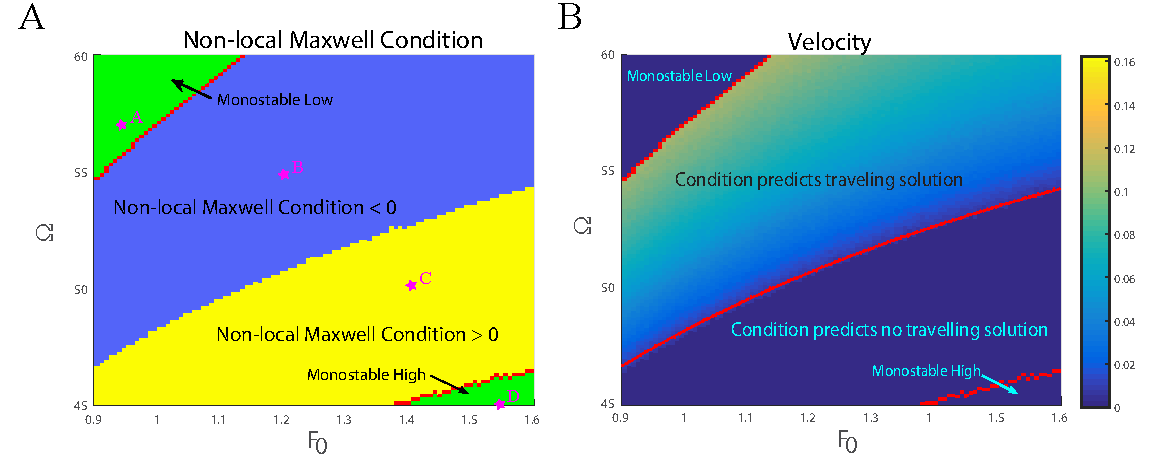
\includegraphics[width=6in]{Project2/figs/MM_results.pdf}
\caption{(A)The results of varying two parameters $\Omega$ and $F$ and the regions where the non-local Maxwell condition is either greater than $0$ (yellow) or less that $0$ (blue). Red lines indicate the boundaries between the monostable and bistable regimes. The pink stars correspond to locations in parameter space where the corresponding phaseline plots of Fig.~\ref{fig::phaseline} were made.  (B) Velocity resulting from numerical solutions of the PDE as two parameters are varied. Red lines indicate the boundaries between the monostable and bistable regimes, as well as the line across which the non-local Maxwell condition is equal to $0$.}
\label{fig::NLMC}
\end{figure}




